\documentclass[10pt,twocolumn,letterpaper]{article}

\usepackage{cvpr}
\usepackage{times}
\usepackage{epsfig}
\usepackage{graphicx}
\usepackage{amsmath}
\usepackage{amssymb}


% Include other packages here, before hyperref.

% If you comment hyperref and then uncomment it, you should delete
% egpaper.aux before re-running latex.  (Or just hit 'q' on the first latex
% run, let it finish, and you should be clear).
\usepackage[breaklinks=true,bookmarks=false]{hyperref}

\cvprfinalcopy % *** Uncomment this line for the final submission

\def\cvprPaperID{****} % *** Enter the CVPR Paper ID here
\def\httilde{\mbox{\tt\raisebox{-.5ex}{\symbol{126}}}}

\renewcommand{\arraystretch}{1.4}

% Pages are numbered in submission mode, and unnumbered in camera-ready
%\ifcvprfinal\pagestyle{empty}\fi
\setcounter{page}{1}
\begin{document}

%%%%%%%%% TITLE
\title{Hierarchical Multiclass Object Classification }

\author{Fereshte Khani\\ 
  Massachusetts Institute of Technology\\
  {\tt\small fereshte@mit.edu}
  % For a paper whose authors are all at the same institution,
  % omit the following lines up until the closing ``}''.
  % Additional authors and addresses can be added with ``\and'',
  % just like the second author.
  % To save space, use either the email address or home page, not both
  \and
  Anurag Mukkara\\
  Massachusetts Institute of Technology\\
  {\tt\small anurag\_m@mit.edu}
}

% TODO
% spell check
% bold text for variables


\maketitle
%\thispagestyle{empty}

%%%%%%%%% ABSTRACT
\begin{abstract}
  
Humans can use similarity between objects in order to recognize rare objects.
They also make many abstract concepts when they see some objects very often.
Interestingly, a large part of brain is associated with common classes like
faces rather than rare objects like Ostrich.  In our work we want to propose
a model that has four mentioned characteristics. 1. Use more resources for
categories that have many examples and less resources for categories that
have few examples, 2. Has the ability recognize objects that it has never
seen before, but can be synthesized by combining previously seen objects, 3.
Objects with few examples can borrow statistical strength from similar
objects with many examples, 4. Models that have lot of sharing between model
parameters of different classes should be favored.
  
\end{abstract}

%%%%%%%%% BODY TEXT
\section{Introduction}

Object classification is one of the fundamental problems in computer vision.
It becomes a lot harder when number of categories is large. When number of
categories is very large, the complexity of the model should not be related to
the number of categories. It should capture the similarities between categories
in order to classify objects in an easier and more accurate way.

We all have a hierarchy based abstraction for recognizing objects around
us. We make more hierarchical concepts for object that we encounter more often.
For example, if you ask a person about furniture they can categorize it by
chair, desk, sofa, table, etc. and then for chair it goes like office chair,
armchair, rock chair, or even wheelchair. These sub categories are related
to each other visually. In this work, we try to propose a model that makes
more abstract concepts when there are lots of similar classes and less
otherwise. This model also share many parameters between similar objects.
It helps rare objects that we have less training example from them use
parameters of common examples. In other words, common classes have lots of
training example by these examples algorithm can set accurate parameters.
On other hand, rare objects have very few examples and set the parameters
in an accurate way is almost impossible . Sharing parameters between these
classes help rare classes to borrow statistical strength from common
classes. 

We all make a model for every concept and when we encounter a new object we try to
check to which concept model it matches more. All learning algorithms try to add
additional information to the problem to avoid over fitting. They usually use
Occam-razor to have models as simple as possible. Here we want to
change this regularization in a way that if a model uses previously learned
objects it can have more complex shape. By this structure, models that have lot
of sharing between model parameters of different classes will be favored.

There are many objects around us. In the model that we have many categories,
when we want to train a classifier to learn objects we should be able to
model the similarities between different categories otherwise we should
store a lot of redundant information. In one vs all methods there is no
difference between bicycle vs motorcycle and dogs vs motorcycle. While we
like that if we have a false positive it should be bicycle rather than dogs. 
Even humans sometimes are confused between different dogs or wrongly
assume another animal to be a dog. So, we want a classifier to model this
similarities.  

The rest of paper is as follows, in section 2 we give an overview of related work.
There is an overview about independent multiclass classification in section 3. In
section 4 we explain our method which is a hierarchical multi-class model for
object recognition. We discuss experimental results in section 4 and conclude 
in section 5.


\section{Related work}

There are lots of work being done in the field of transfer learning in object
classification. There are three main questions that people should answer when
they want to use transfer learning. 1) What to transfer?,  2) How to transfer?,
When to transfer?. For a good survey in transfer learning see
\cite{transfersurvey}. For the first question, there are methods that share
parameters between classes like you can learn parameter of deep network
\cite{deepnet} by Imagenet \cite{imagenet} and then test it in on another
benchmark. One other method is sharing training examples.  One important
thing in how we should transfer is that between which classes we should
transfer parameters/features. For example when we add a new class we
should decide that with which classes this class should share features.
If there are only a few examples from each class so deciding which
classes should share information and which classes should not is a hard
question.

For finding which classes should share information some methods use a global
priori \cite{priori} (share information between all classes) which provides
small benefits but still is better than independent classifiers. There are some
models \cite{semantic} that use an external hierarchy. For example, in
\cite{semantic}, wordnet \cite{wordnet} is a semantic network for English
language. Words are grouped together if they are synonyms and record semantic
relation between them. With this dictionary one can understand both bicycle and
care belong to vehicle.


Ruslan et al. \cite{ruslan} make a tree in which every class is a leaf. In
their setting, height of tree is fixed and is equal to two. However, number of
super-categories in the tree is not fixed and they use Chinese Restaurant Prior 
to decide if they should add
a new super-category to the tree or not. Classes which have a common parent share
features. They add classes incrementally to the tree. At each step they decide
where in the tree they should place the new class. Although this setting support
feature 3, it does not incorporate the other features mentioned above. 
Ruslan et al. improve  their model in \cite{ruslan2} with deep network features.

Sivic et al. \cite{sivic} group images using multi-layer hierarchy tree. Tree
is based on common visual elements. They used generative Hierarchical Latent
Dirichlet Allocation(hLDA)\cite{hlda}. This model is usually used for unsupervised learning of topic
hierarchies. In their work, they automatically (without supervision) discover a
hierarchical structure for the visual world using unlabeled images. They are
also some models that try to find some relation between categories and use them
to classify images \cite{transfer22}.
For the last question that when we should transfer, algorithms deal with questions like this: should we use transfer information just for testing or we can use them for training as well? If we want to use transfer information during learning should we use them at first or in the middle? Another main issue in this area is that when it is good to transfer information, and when it make it worse when we transfer information. See \cite{whentransfer} for more details.

%In \cite{wordnet} 
%There are papers that use hierarchical for sharing features and parameters between classifiers. f
%There are many algorithms in the field of transfer learning in multi class object %recognition.(\cite{miller2000learning}) 


\section{Hierarchical Classification Model}

\subsection{Learning Independent Classification Models}

Consider a classification problem where we observe a dataset $D$ of labeled  training examples. 
Each example belongs belongs to one $K$ classes(eg. 40 object categories). The dataset $D$
has $n_{k}$ labeled examples for for each class $k  \in {1,2,....,K} $. We $x_{i}^{(k)} \in R^{D} $ 
be the input feature vector of length D for the $i^{th}$ training example of class $k$ and 
$y_{i}^{(k)}$ be the corresponding class label. $ y_{i}^{k} = 1 $ indicates that the $i^{th}$ training example 
is a positive example for class $K$ and  $ y_{i}^{k} = -1 $ indicates that the $i^{th}$ training example 
is a negative example for class $K$.

For a binary classification problem we can use a simple logistic regression model. In particular, 
for each class $k$, the probability of a positive instance can be modeled as: 
\begin{equation}
  p(y_{i}^{(k)} = 1 | \beta^{(k)} )  = \frac { \exp( \beta^{(k)^{T}}  x_{i}^{(k)})  }{  1 + \exp(\beta^{(k)^{T}}  x_{i}^{(k)} ) } 
\end{equation}
where $k$ ranges over the $K$ classes and $ \beta^{k}  \in R^{D} $ is the unknown model parameter of length D 
for class k. 
In addition, we place a zero-mean spherical Gaussian prior over each model parameter  $  \beta^{k} $:
\begin{equation}
  p(\beta)  = \prod_{k=1}^{K} p(\beta^{(k)}) = \prod_{k=1}^{K} N(0, \frac{1}{\lambda})
\end{equation}
where $N(\mu, \Sigma)$ indicates a Gaussian probability distribution with mean $\mu$ and covariance $\Sigma$.
Here, $\lambda$ is the prior parameter.  With this modeling framework, the log posterior distribution of the unknown 
parameters can be expresses as 
\begin{equation}
  \log p(\beta | D) \propto \sum_{k=1}^{K} \Big[ \, \ \sum_{i=1}^{n_{k}} \log p(y_{i}^{(k)} | x_{i}^{(k)}, \beta^{(k)}) \ + \ \log p(\beta^{(k)}) \ \Big] \,
\end{equation}
Maximizing the log posterior(or finding the MAP estimate ) over the unknown model parameters $\beta$  is  equivalent to 
minimizing the probabilistic loss function with quadratic regularization terms:
\begin{equation}
  E = \sum_{k=1}^{K}  \Big[ \, \ \sum_{i=1}^{n_{k}} Loss(y_{i}^{(k)}, x_{i}^{(k)}, \beta^{(k)}) + \frac{\lambda}{2} \| \beta^{(k)}) \|^{2} \ \Big] \,
\end{equation} 
where the probabilistic loss function is given by:
\begin{equation}
  %Loss(y_{i}^{(k)},  x_{i}^{(k)},  \beta^{(k)})  =  - \sum_{j \in {-1,1} } I\{y_{i}^{(k)}=j\} \log p(y_{i}^{(k)}=j | x_{i}^{(k)},\beta^{(k)})
  Loss(y,  x,  \beta)  =  - \sum_{j \in {-1,1} } I\{y=j\} \log p(y=j | x,\beta)
\end{equation} 
One important property of the loss function is that it is convex and hence can be efficiently optimized
using standard convex optimization solvers.

The main drawback of this formulation is that all the $K$ classes are treated as unrelated entities and hence 
do not share any model parameters. In fact, it is observed that the objective function decomposes into 
$K$ sub-problems, each of which is a binary classification problem that can be trained independently 
using the training data for that particular class.


\subsection{Learning a Hierarchical Classification Model}

\begin{figure}[t]
 	\begin{center}
 		%\fbox{\rule{0pt}{2in} \rule{0.9\linewidth}{0pt}}
 		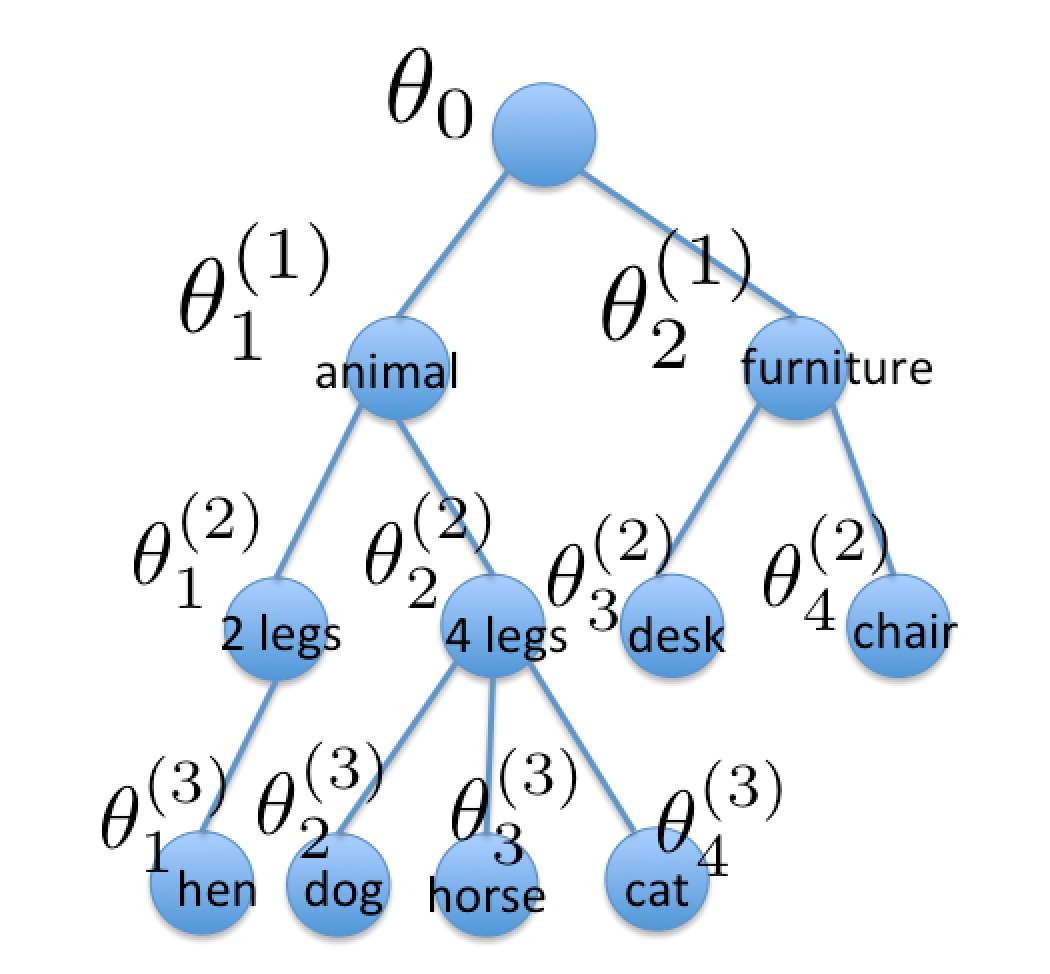
\includegraphics[width=0.8\linewidth]{tree_withoutnew.png}
 	\end{center}
 	\caption{Hierarchical Classification Model with trees of arbitrary height.
 	         Each node in the tree has a model parameter associated with it.
 	         The leaf nodes correspond to various classes and the non-leaf nodes
 	         are the super-categories. Model parameters for each class
 	         are given by the sum of parameters along the path from the 
 	         corresponding leaf node to the root node}
 	\label{fig:hier-tree-intro}
 \end{figure}

In our framework, a hierarchical tree structure, depicted in Fig.~\ref{fig:hier-tree-intro} is used to model sharing of parameters between 
visually related classes. Each node in the tree has a model parameter, a vector of length $D$ 
associated with it.  Let $ \theta = \{ \theta_{1}, \theta_{2},.....,\theta_{n}\} $ denote the model parameters 
of all the nodes in the tree, where $n$ is the number of nodes starting from the root node to the all the leaf nodes.
The leaf nodes correspond to the $K$ object categories or classes. The parameters for a particular class $k$
is the sum of the parameters of all the nodes, say $i_{1}, i_{2}, ..., i_{l} $, along the path from the leaf node
corresponding to that class up until the root node of the tree:
\begin{equation} \label{beta-theta-rel}
  \beta^{(k)} = \theta_{i_{1}} +  \theta_{i_{2}} + ...... + \theta_{i_{l}}
\end{equation} 
We place zero-mean spherical Gaussian priors on the parameters of each node. However, the 
covariance matrix is dependent on the level of a particular node in the tree i.e all the nodes at
a particular level have the same prior parameters.
\begin{equation}
  p(\theta_{i})  = N(0,\frac{1}{\lambda_{l}}I) 
\end{equation}   
where node $i$ is at level $l$ in the tree. The root node has level 0 and the level increases as 
we move towards the leaf nodes.

With this modification in the way the model parameters for classes are related,  the hierarchical 
learning problem can be formulated as minimizing the log posterior or equivalently the loss function 
with respect to $\beta$:
\begin{equation} \label{hier-loss}
  \begin{split}
    E = Loss(Y,X,\beta) + \frac{\lambda_{0}}{2} \|\theta_{0} \|^{2} +
    \sum_{i=1}^{k_{1}} \frac{\lambda_{1}}{2} \|\theta_{i1} \|^{2} & \\
    + \sum_{i=1}^{k_{2}} \frac{\lambda_{2}}{2} \|\theta_{i2} \|^{2} +
    ...... +
    \sum_{i=1}^{k_{l}} \frac{\lambda_{l}}{2} \|\theta_{il} \|^{2} &
  \end{split}
\end{equation} 
 where $Loss(Y,X,\beta)$ is the loss function as explained in the previous section
 but with the additional constraint that $\beta$ satisfies  equation \ref{beta-theta-rel} 
 according to the tree structure. Here there are $k_{j}$ nodes in level $j$ and 
 $\theta_{1j}, \theta_{2j},.....,\theta_{k_{j}j}$ are the parameters of nodes in level $j$.

\subsection{Learning the tree structure}
 
If we are given the tree structure that indicates the relation between different classes, then the 
learning algorithm only needs to optimize for the loss in equation \ref{hier-loss}. However, as 
discussed in \cite{ruslan}, learning the tree structure dynamically based on the input classes and training data
could lead to better results in object classification. We adopt the algorithm used in \cite{ruslan} to multilevel trees
and fine-grained partitioning. In \cite{ruslan}, the author use a fixed number of levels i.e 3 in the tree and use
a non-parametric Chinese Restaurant Process Prior(CRP) to model the position of a class in the tree. Although this simple
CRP prior allows one to have unknown and potentially unbounded number of groups of object classes, this is can only be
used for two-level trees. For trees which have a fixed number of levels more than 3, one could use a nested CRP prior \cite{nestedCRP}.
Since this approach has the drawback of limiting the tree to a fixed number of levels, we use a simple extension(modified-CRP) of the
CRP prior used in \cite{ruslan} to allow the flexibility of  having different depths at different parts of the tree.    

\begin{figure}[t]
	\begin{center}
		%\fbox{\rule{0pt}{2in} \rule{0.9\linewidth}{0pt}}
		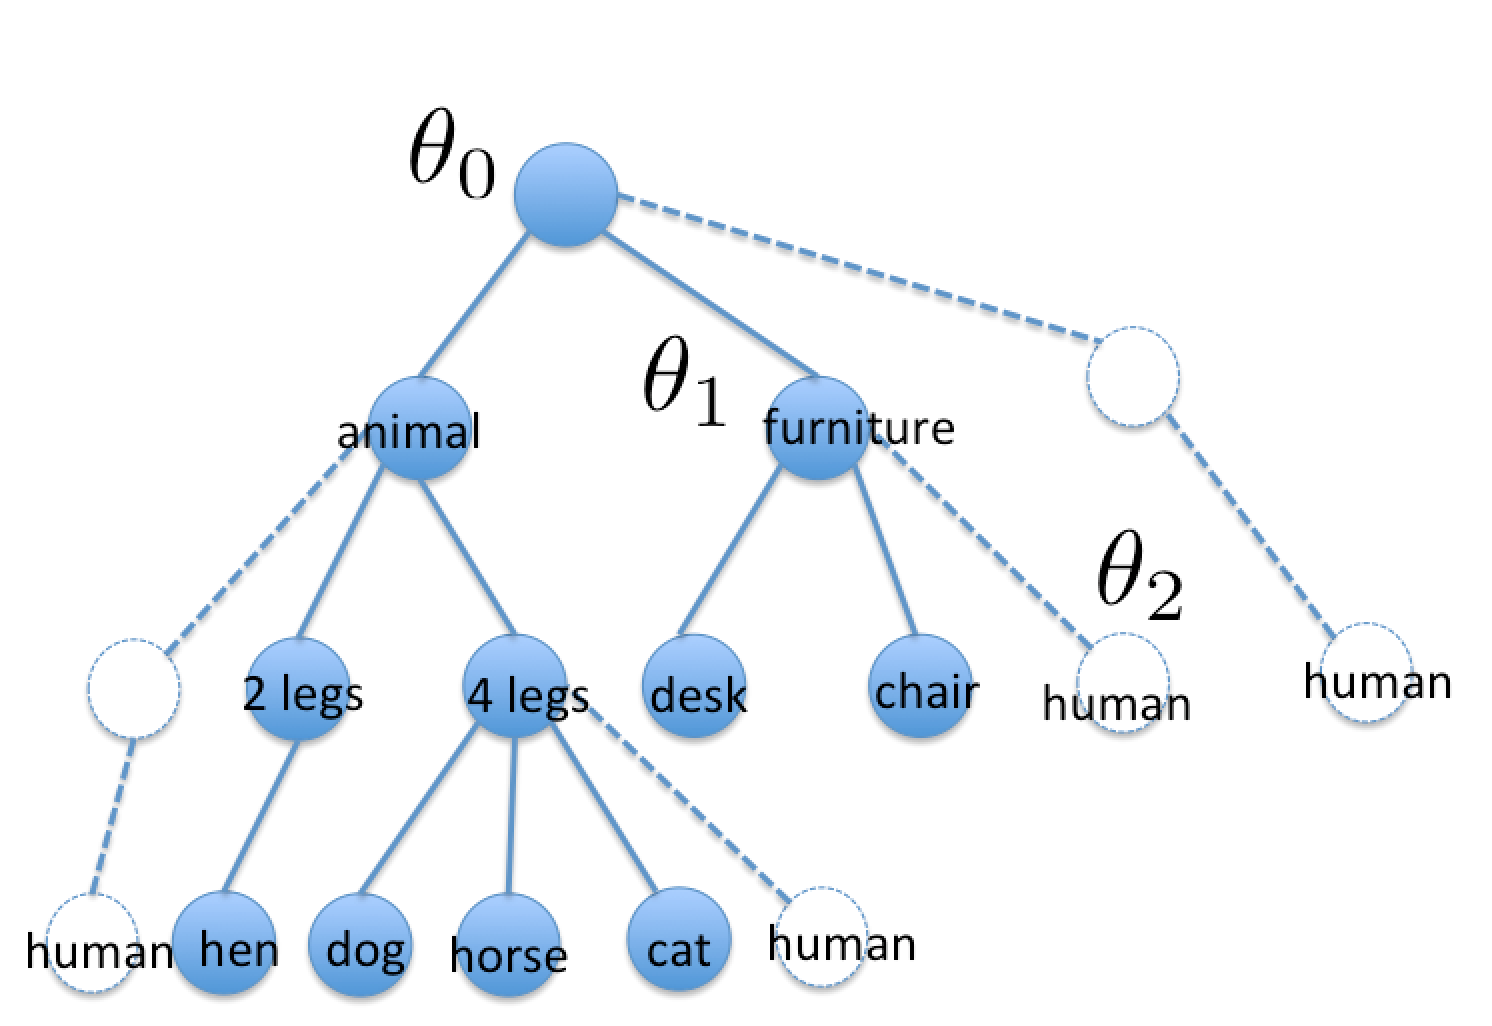
\includegraphics[width=0.8\linewidth]{tree}
	\end{center}
	\caption{ Learning the tree hierarchy. The `human' node can be attached 
              to one of the existing super-categories:`animal', `4-legged animal', `furniture'
              or create its own novel super-category.}
	\label{fig:learning-tree-hierarchy}
\end{figure}



A new class could go into one of the existing super-categories or create a new super-category. A new super-category 
can be attached to any node which doesn't have any children that are leaf nodes. That is, we allow the parent of a new
super-category to be any node that is not itself a super-category that has leaf nodes, which correspond to classes, as children.
An example is shown in Fig.~\ref{fig:learning-tree-hierarchy}.
By following the procedure in \cite{ruslan}, for each possible position of the new class we calculate a likelihood term and 
modified-CRP prior term. The position of the new class will be the one that maximizes the sum of likelihood term and  prior term. 

Let $i$ denote the node number of the leaf node corresponding to the new class.   
To calculate the likelihood at a possible position in the tree, we find the model parameter $\theta_{i}$ of the leaf node, 
that maximizes the log likelihood of the training data at that position. This likelihood will depend on the position in the tree, when 
we choose a position it means that we include the parameters of all the nodes that are ancestors of the leaf node $i$ at that position. 
If the position corresponds to a category that is visually dissimilar to the new class, then the best we can with $\theta_{i}$ with still 
result in a lower likelihood term. If the the category is visually similar to the new class, we can achieve a far better fit and the likelihood
term goes up. We have observed that the maximum of the likelihood over the model parameter $\theta_{i}$ is greatly affected by the position
we choose for the leaf node. In addition to the likelihood term, the modified-CRP prior term favors super-categories that have a large number of 
 leaf nodes or class under them. The modified-CRP prior is given by:
 
 \begin{displaymath}
 p(z=j) = \left \{
	    \begin{array}{lr}
 		\frac{m_{j}}{n+\gamma*m} & : \text{$j$ is old} \\
		\frac{\gamma}{n+\gamma*m} & : \text{$j$ is new}
	   \end{array}
	  \right.
 \end{displaymath} 
 
  
where $n$ is the total number of leaf nodes, $m_{j}$
is the number of leaf nodes under super-category $j$,
$\gamma$ is the concentration parameter that controls the probability of creating a new super-category,
$m$ is the total number of positions of new super-categories in the tree. $m$ is equal to number of nodes
in the tree that have only super-categories as children. In other words, $m$ is the cardinality of the set that 
includes the root node as well all nodes that are not leaf nodes or parents of leaf nodes. It can be easily verified that 
this defines a valid probability distribution over the choice $z$ of possible positions in the tree where the new class can be placed.


We use the same model-fitting algorithm described in \cite{ruslan} with modifications to CRP-prior term and tree structure as described above.
Basically, the algorithm alternates between deciding the position in the tree of a new class and optimizing the model parameters of all the nodes
in the tree for a given tree structure.  This alternating procedure will reach a local minima of the loss function 
described in equation \ref{hier-loss}. Since the loss function is convex, this is also the global minima of the loss function. 
For optimizing the model parameters for a fixed tree structure , we use iterative coordinate-descend procedure.
Since the parameters of all the nodes at any given level of the tree are independent of each other, we parallelize the loss minimization 
routine for these nodes. This leads to significant reduction in time taken to learn the model.

\begin{figure}[t]
  	\begin{center}
  		%\fbox{\rule{0pt}{2in} \rule{0.9\linewidth}{0pt}}
  		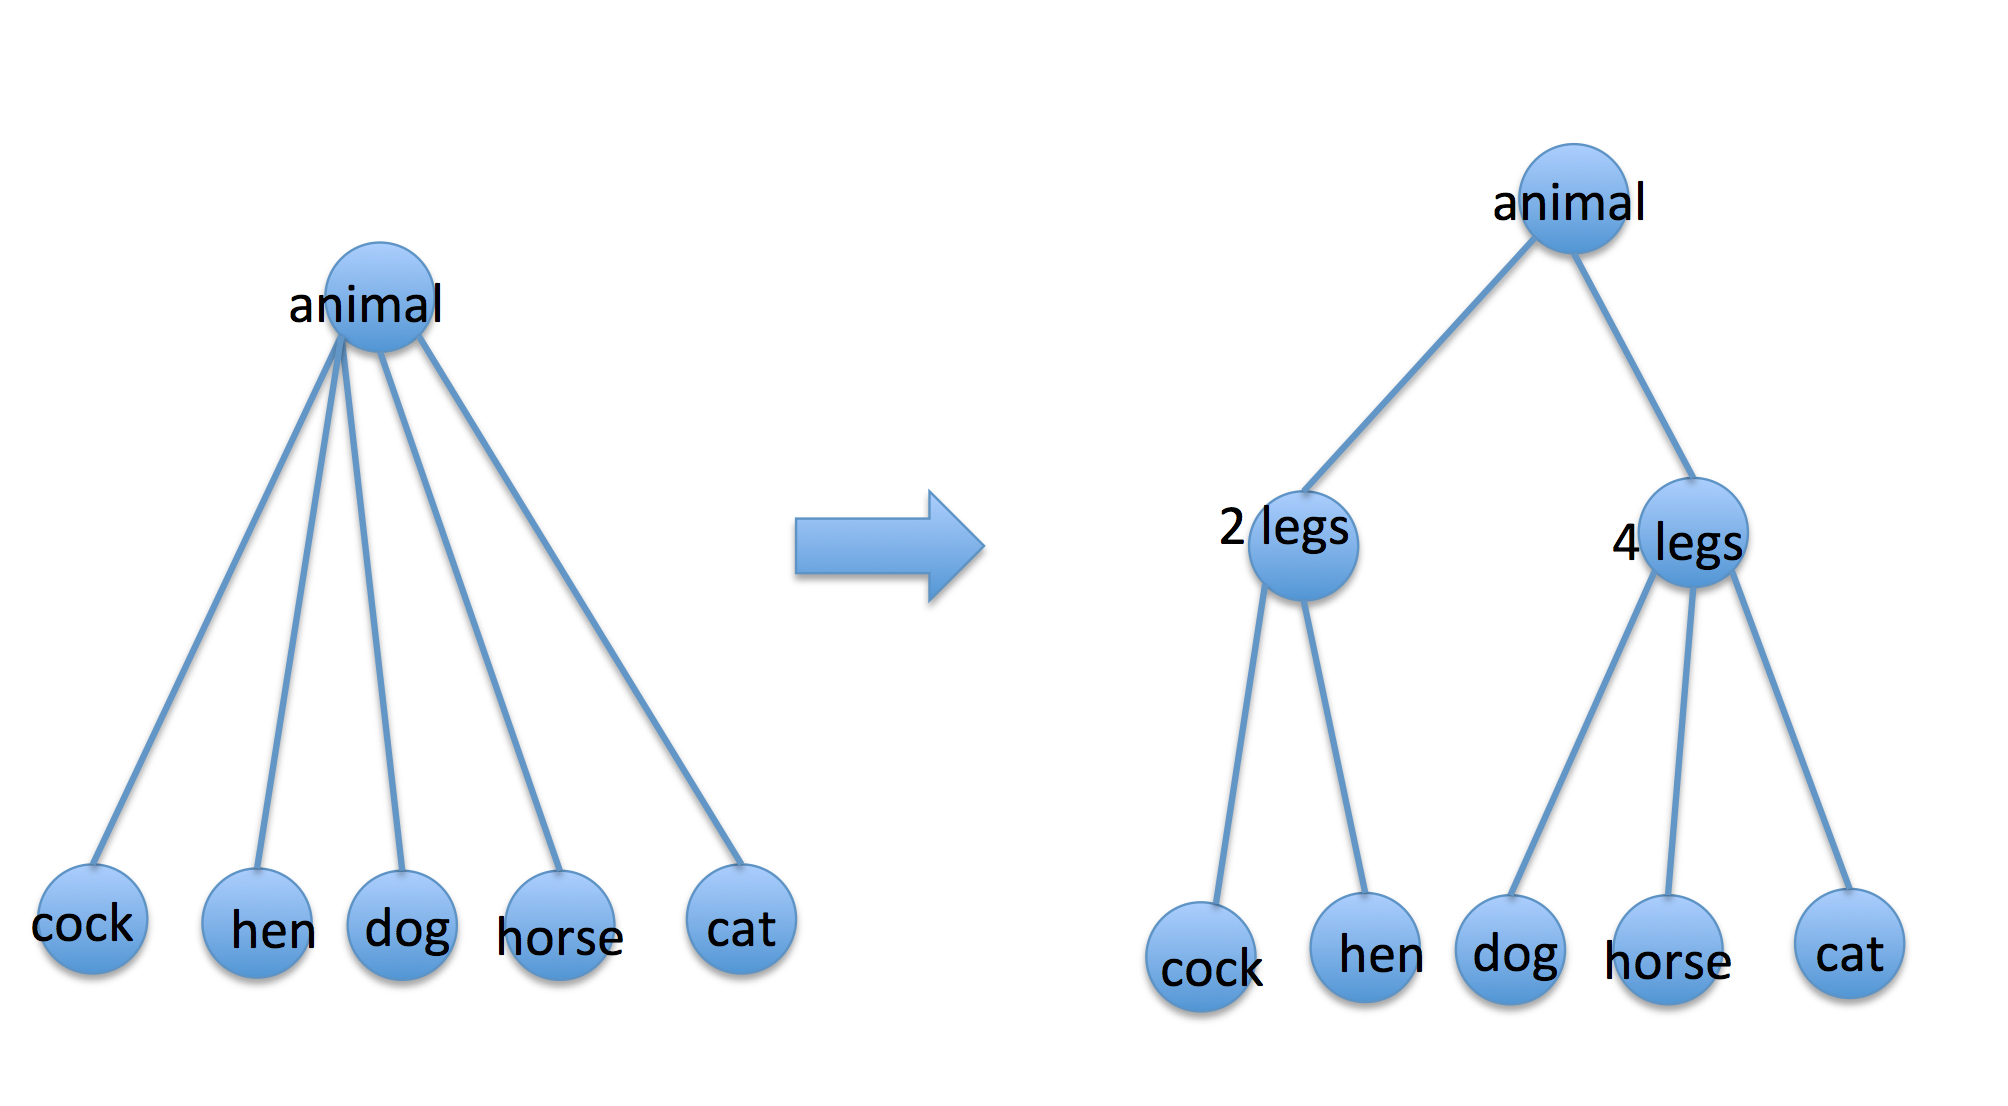
\includegraphics[width=0.8\linewidth]{split}
  	\end{center}
  	\caption{ Maintaining a fine-grained partitioning. When number of nodes under 
              animal super-category goes above maxChild=4, we break the subtree into 
              finer partitions while not disturbing the remaining parts(not shown in figure) 
              of the tree.  }
  	\label{fig:long}
  	\label{fig:onecol}
  \end{figure}


We also use a simple heuristic to maintain a fine-partitioning of the classes among into among super-categories. 
We need to avoid many leaf nodes accumulating under the 
same super-category as this would lead to a very coarse-grain partitioning of the classes.  So, whenever the number of leaf nodes under a 
super-category goes above a certain threshold $maxChild$, we break down the sub tree under that node to create
 a more fine-grained partitioning.  To do this we run the entire optimization algorithm described above on the classes that were originally under this
 super-category. Basically, we consider the node corresponding to the super-category as a root node and keep adding new leaf nodes 
 to form a tree under this root node. In most cases, the $maxChild$ number of classes that previously shared the same parent are dividing
 several finer super-categories and have different parents.  In the rare case when the classes are very similar to each other, this process will add
 redundant to the tree. We identify this pathology and remove the redundant node while appropriately modifying the model parameters of the 
 relevant nodes. The parameter $maxChild$ can be configured to control the degree of fine-grained partitioning of classes. A lower value
 of $maxChild$ leads to very fine-grained partitions whereas a higher value of $maxChild$ results in coarser partitions. We found that 
 a value of four results in best results. 
 
 \begin{figure}[t]
 	\begin{center}
 		%\fbox{\rule{0pt}{2in} \rule{0.9\linewidth}{0pt}}
 		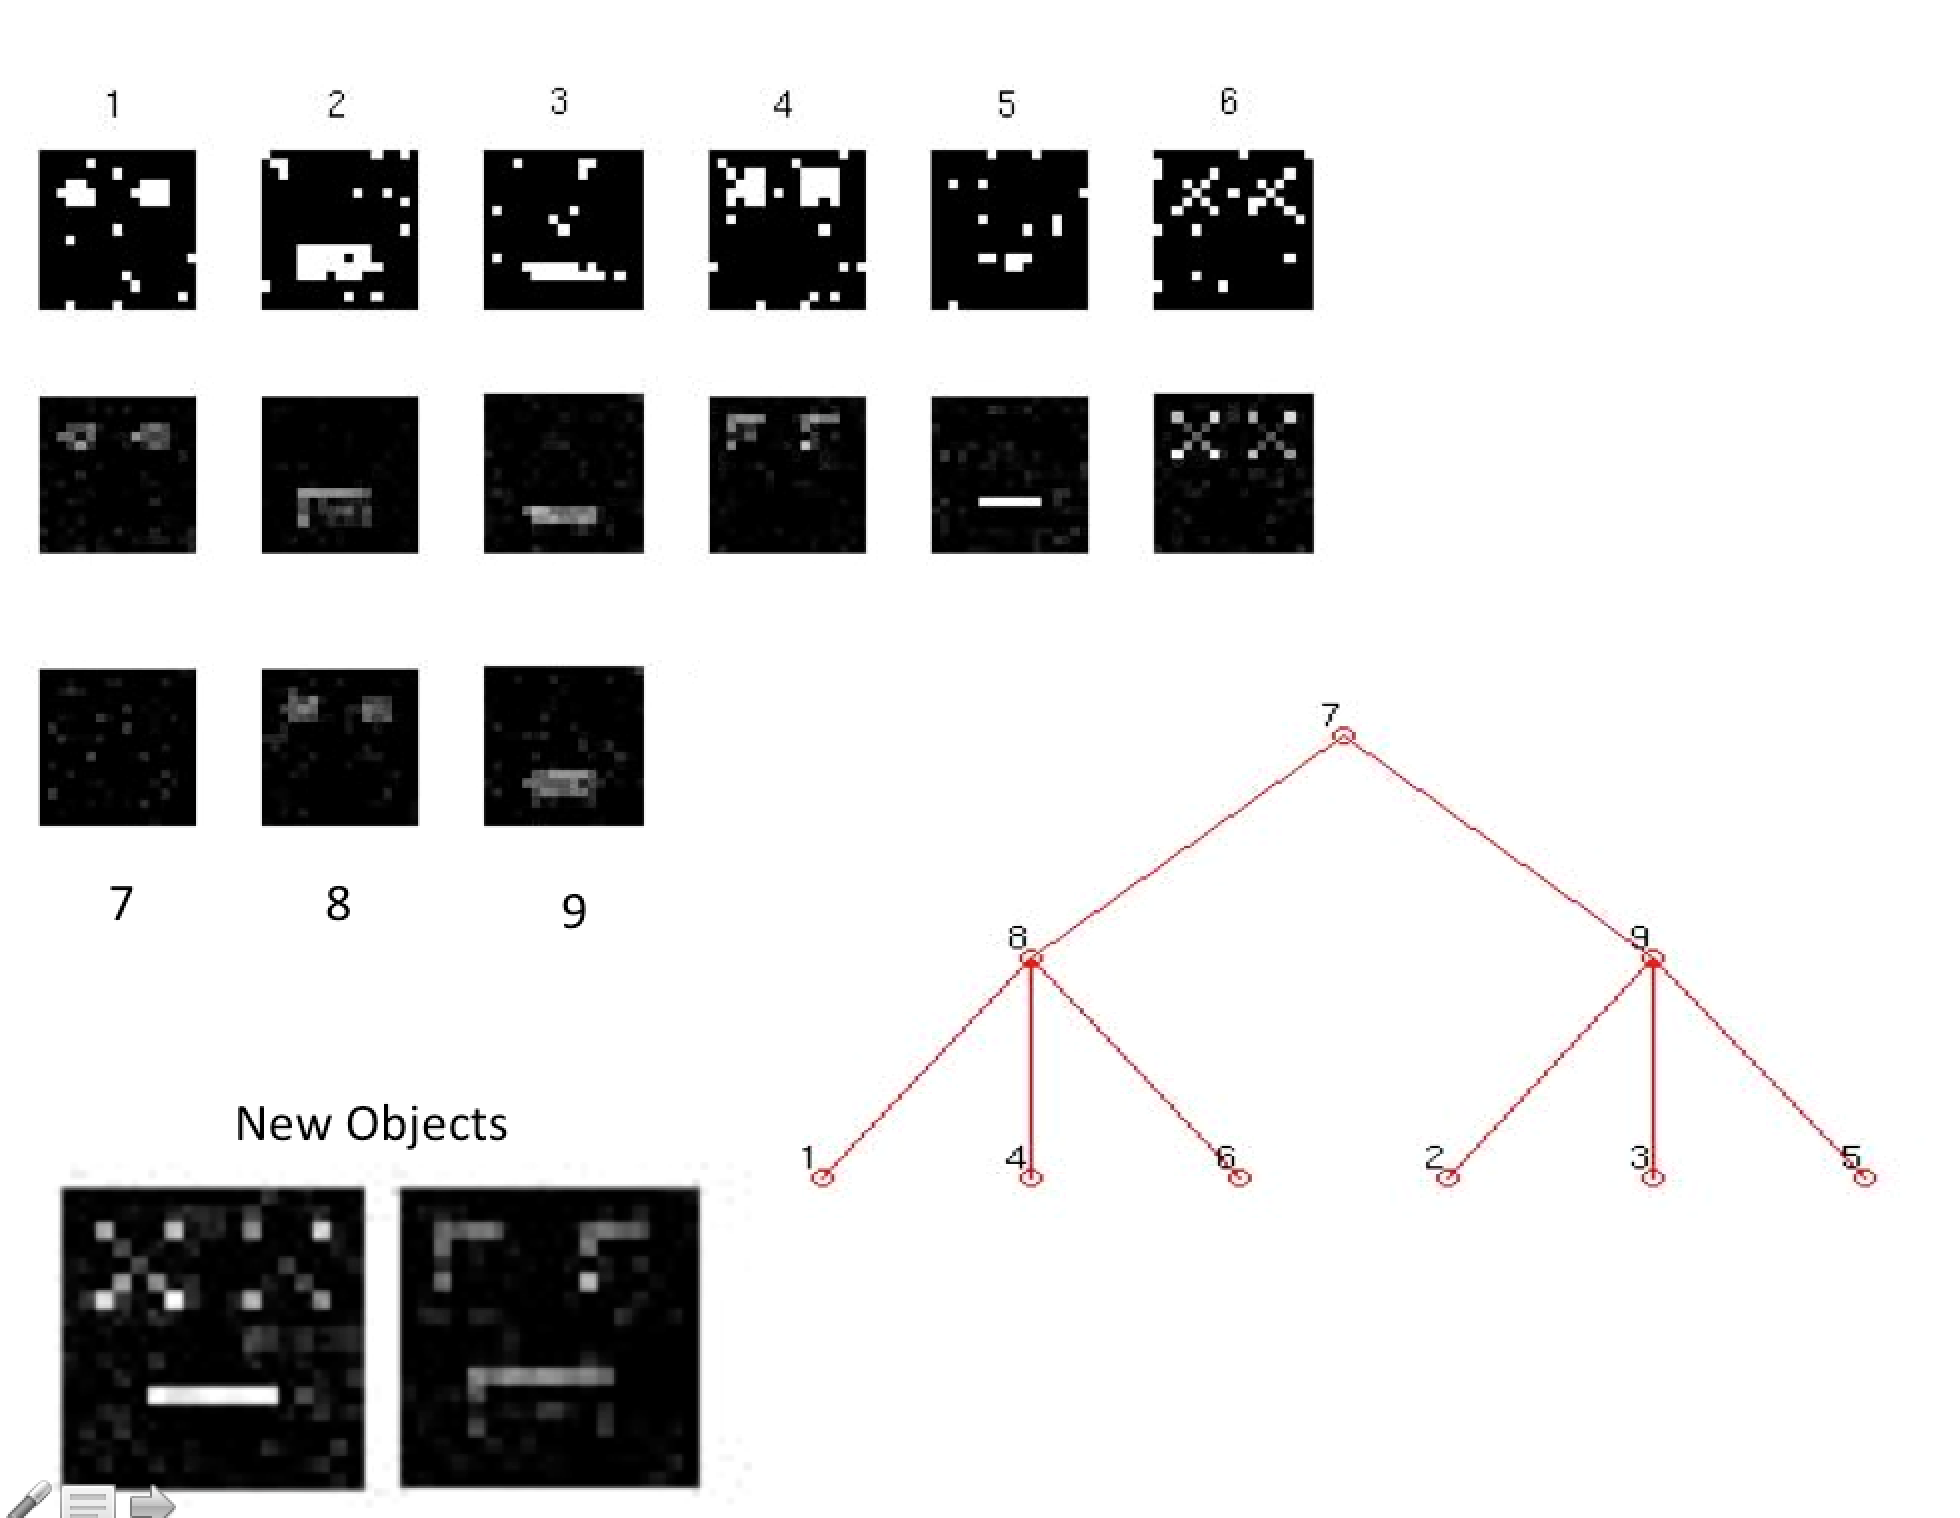
\includegraphics[width=0.9\linewidth]{smiley}
 	\end{center}
 	\caption{(a) First row shows eight classes of smiley faces. class 1,4,6 just have eyes and class 2,3,5 just have eyes. The second row show the visualization for parameter $\theta$ for each node. The third line shows the visualization of $\theta$ for node 7,8,8 respectively. (b) shows the tree corresponding to these examples. As you can see in the visualization of parameter of node 7,8 they capture that there are eyes or mouths in their children. (c) shows two visualization of smiley faces by adding parameter by adding parameter $\theta$ of different nodes. If a new example which is look like these two come for testing we can identify it by these two}
 	\label{fig:smiley}
 %	\label{smiley}
 \end{figure}
\section {Experiments}
 
 \begin{figure}[t]
 	\begin{center}
 		%\fbox{\rule{0pt}{2in} \rule{0.9\linewidth}{0pt}}
 		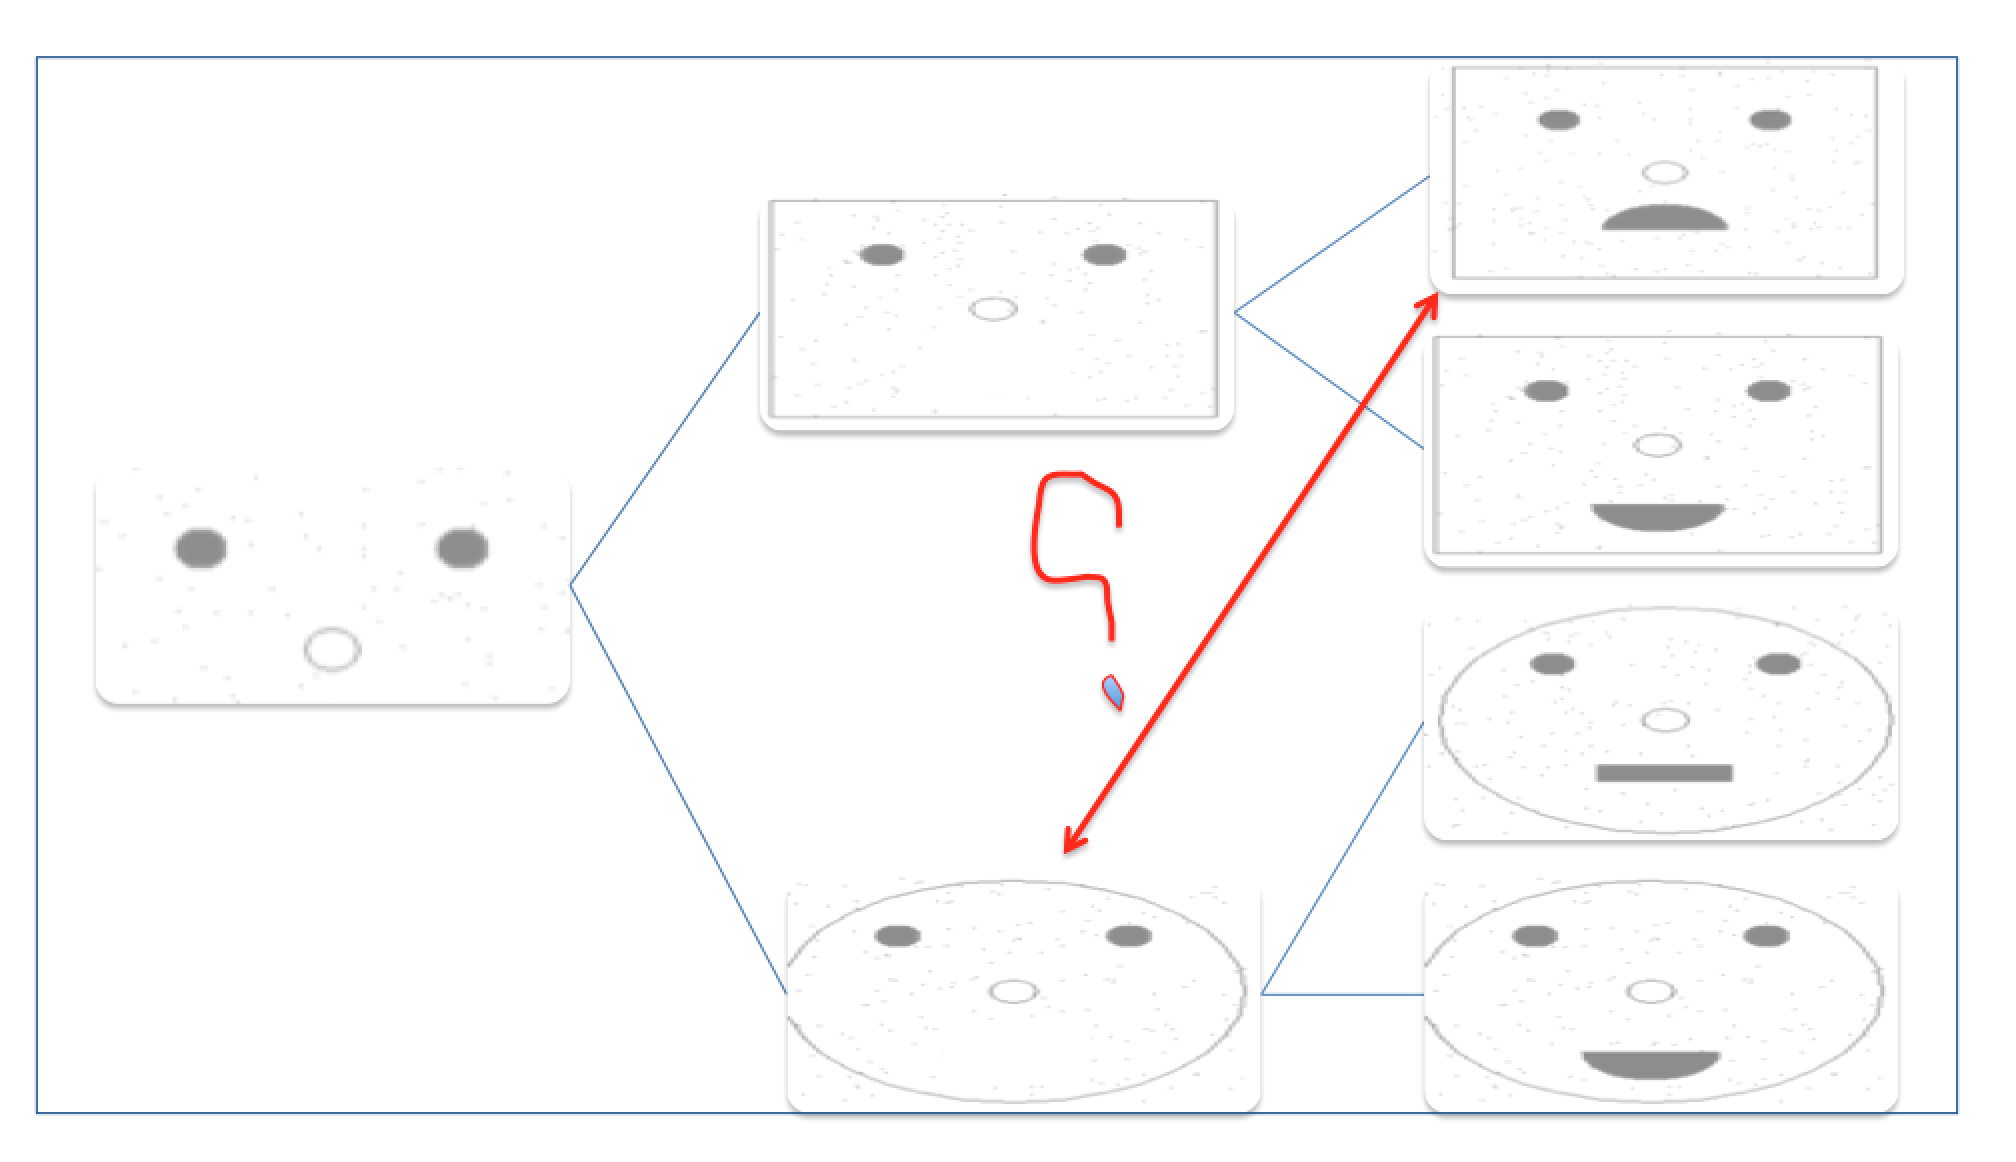
\includegraphics[width=0.6\linewidth]{merge}
 	\end{center}
 	\caption{We propose a model that can combine features of two different classes to make a new class. In this figure, the goal is to recognize sad circle face by just training on smiley circle face and sad square face}
 %	\label{fig:long}
 	\label{merge}
 \end{figure}
 
 
 \subsection {Implementation}
 We implemented the whole algorithm in MATLAB.  The code is available at \cite{website:sourceCode}. We use HOG \cite{hog} to generate feature vectors for images. 
 For optimizing the probabilistic loss functions we use \textit{fminunc} function in MATLAB that does unconstrained optimization using Quasi-Newton method. 
 One can use HOGgles \cite{hoggles} in order to visualize the learned model parameters.
 
At testing time, we decide the class of an input image as the one that has the maximum probability
for the learned model parameters.
\begin{displaymath}
 \text{predictedClass} = \operatorname*{arg\,max}_{k} \frac { \exp( \beta^{(k)^{T}}  \phi(x^{(k)}))  }{  1 + \exp(\beta^{(k)^{T}}  \phi(x^{(k)}) ) }
\end{displaymath}  
 
 \subsection{Data Sets}
 \subsubsection{Smiley Faces}
 We make a syntactic data set in order to check our algorithm's properties(merging two subcategories, make meaningful abstract concepts, make more nodes when there are more classes). There are 320 classes in this data set. Each class is a smiley face that has different nose, mouth, face and eyes. There are 1000 positive and 1000 negative examples in each classes. The pictures are 25 by 25 and we add random noise to each example of the class.
  
 \subsubsection{Fine Grained Data Set}
 We use data set of Fine Grained Challenge \cite{dataSet}. There are five different domains (Cars, Birds, Aircrafts, Shoes and dogs) in this data set. In each domain there are about 100 classes. Classes within a domain are very similar to each other like different types of cars, dogs and etc.
 \subsection{Results}
 \subsubsection{Smiley Faces}
 
 As mentioned before, the main reason for making this dataset was to visualize our algorithm's abilities. You can see two abilities of model in Fig.~\ref{fig:smiley}.
 
\textbf{Merging:} As shown in Fig.~\ref{merge} the goal of merging is to create and recognize some objects that we have never seen before but which can be made by combining objects from classes in the training set. In Fig.~\ref{merge} we want to recognize sad circle face by just training on sad square face and happy circle face.

As shown in Fig.~\ref{fig:smiley} we have six classes three of them just have eyes and three of them just have mouths. When we add theta of class 
 
\textbf{Meaningful super categories} As showed in Fig.~\ref{fig:smiley} you can see that when we visualize the model parameters of node 7 we can see that it captures the fact that there are eyes in all its child classes. Same is true for node 8 that captures presence of mouth in all its children.

The accuracy of our algorithm for Smiley faces is 95\%.
   
 \begin{figure}[t]
 	\begin{center}
 		%\fbox{\rule{0pt}{2in} \rule{0.9\linewidth}{0pt}}
 		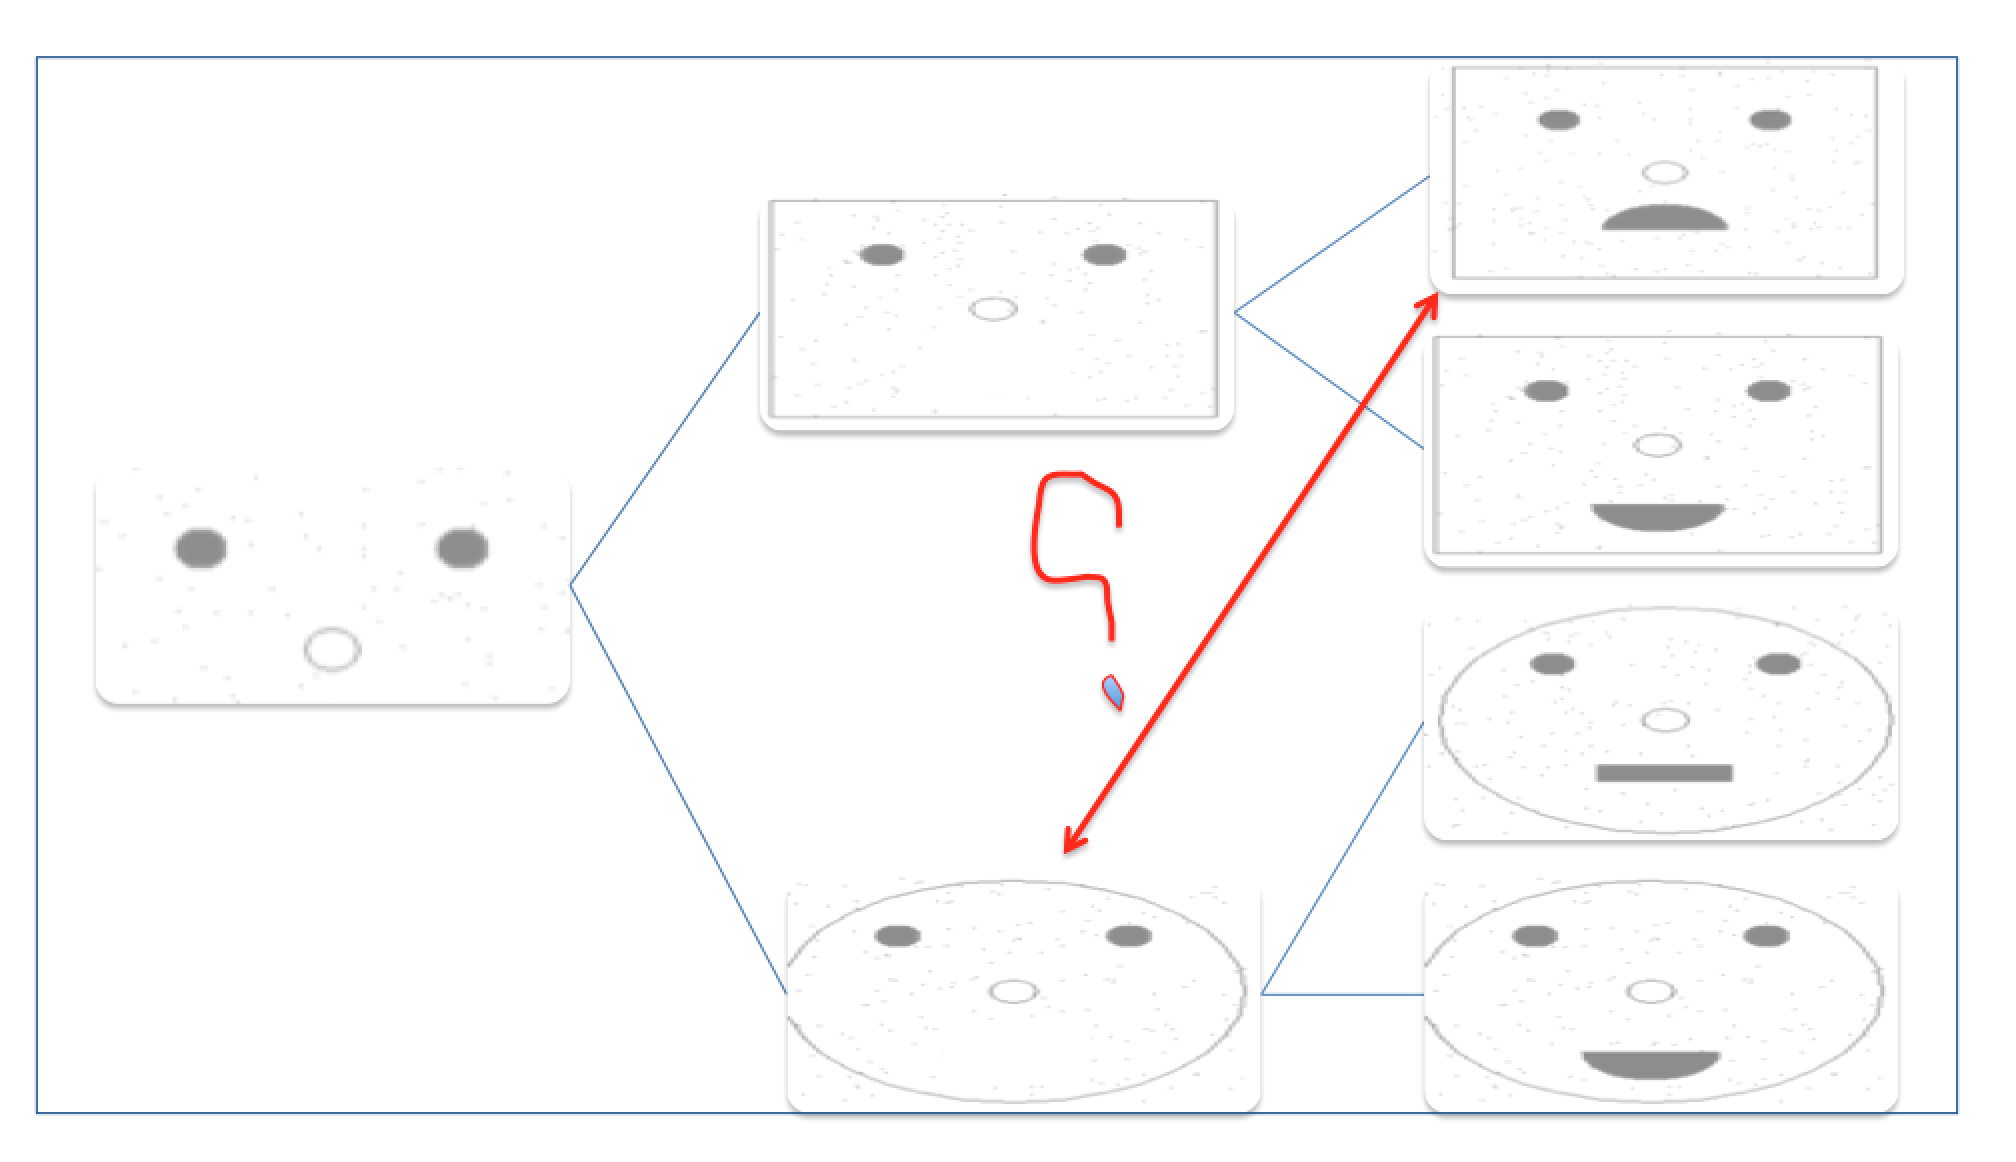
\includegraphics[width=0.8\linewidth]{merge}
 	\end{center}
 	\caption{What question in the filed of computer vision is that how we can combine features of two different classes. In this work we propose a model that we can combine features of two different classes two make a new class. In this figure the goal is to recognize sad circle face by just training on smiley circle face and sad square face}
 %	\label{fig:long}
 	\label{merge}
 \end{figure}
 
\begin{figure*}
	\begin{center}
	%	\fbox{\rule{0pt}{2in} \rule{.9\linewidth}{0pt}}
	    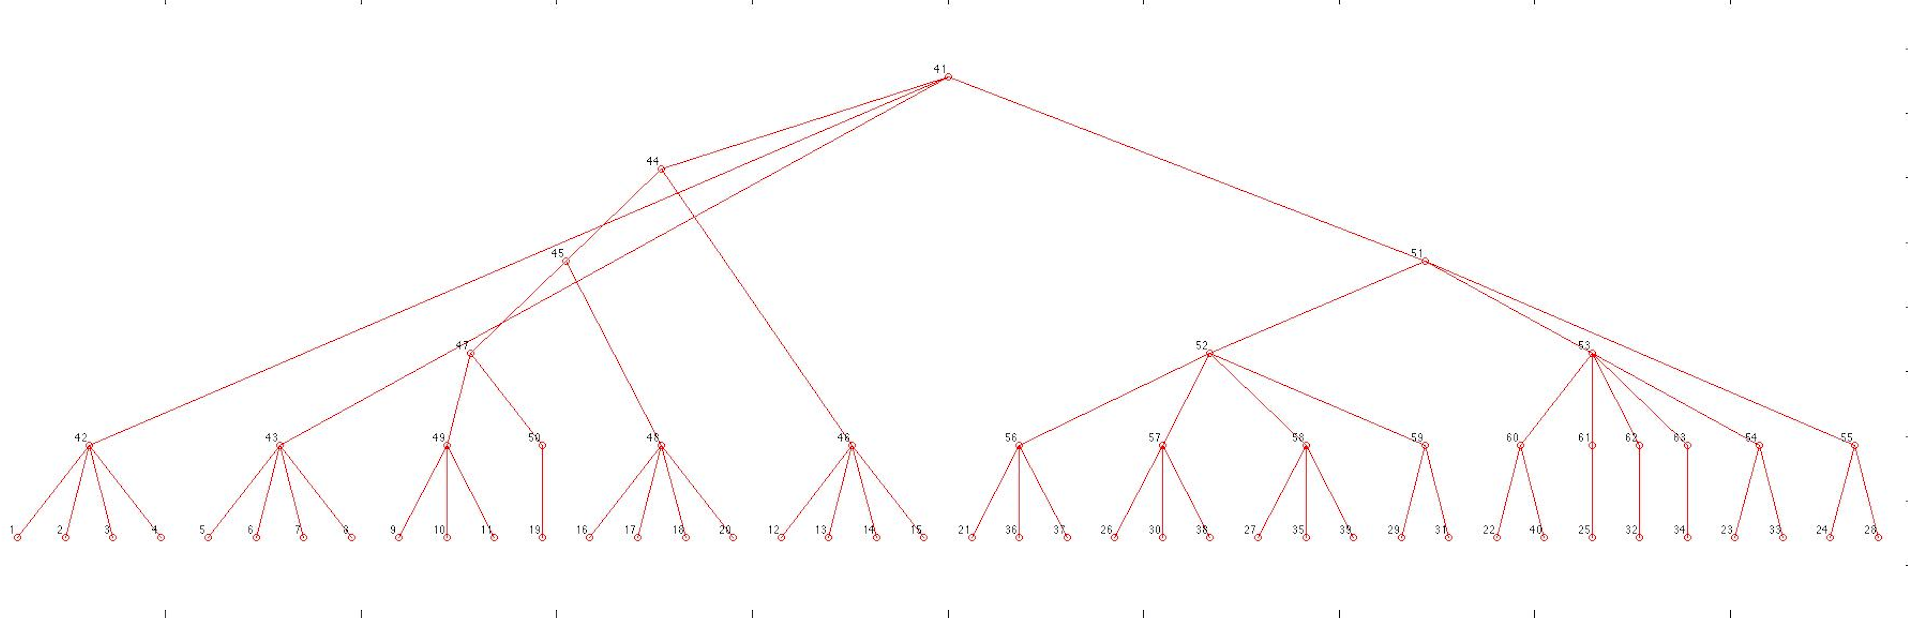
\includegraphics[width=1\linewidth]{carsDogs.png}
	\end{center}
	\caption{This is the tree made by algorithm for fine grained data set, There are two main subtree in the figure the left one corrospond to cars and the right one corrosponds to dogs. Visually simillar dogs/cars are in a same subtree.}
	\label{cardogs}
\end{figure*}

 \subsubsection{Fine Grained Data Set}
 The difference between classes in the same domain is very negligible in this data set. Because of this, finding a good model parameters
 when training on these classes requires high quality pictures and lots of training examples. For example, if we set size of images to 100*100 pixels we can reach accuracy of 70\% for 8 different classes. However, if we set the image size to 50*50 pixels the accuracy decreases to 22\% and 18\% if we set the size to 30*30 pixels.
 
 As the difference between classes are very fine-grained taking into account the color of the image is really important. In our case we find the HOG feature for colored image, however hog is kind of invariant to the color so we miss some information here. We expect that if we include the 3 color channels in the calculating the feature vector for each image we will attain better accuracy.
 
 The accuracy of our model for finding differences between two domains is very high around 92\%, and as you can see in Fig.~\ref{cardogs} cars and dogs belongs to two different sub trees. One other important aspect of our algorithm as we said before we want incorrect examples belongs to similar categories rather than completely different categories. We saw this behavior in our testing.
 
\section{Conclusion}
In this work we try to make a hierarchical presentation of fine grained objects. We test our model on synthetic images and natural images. The algorithm put classes under the same super category if they are visually simillar. The algorithm allows super categories which have lots of classes to have more complex model. As a result, model become more accurate for common objects and rare objects use parameters of common objects for their model.
 




{\small
\bibliographystyle{ieee}
\bibliography{finalReport}
}

\end{document}
